\documentclass[10pt, a4paper, onecolumn]{scrartcl}
\usepackage{cite}  
\usepackage{times}
\usepackage{amsmath}
\usepackage{amsfonts}
\usepackage{amssymb}
\usepackage{graphicx}
\usepackage{listings}
\usepackage{enumitem} % used for list - no spaces between items
\usepackage[english]{babel} % English language/hyphenation
\usepackage[top=2cm, bottom= 3.2cm, left=2cm, right=2cm, columnsep=0.6cm]{geometry}
\usepackage{color} %red, green, blue, yellow, cyan, magenta, black, white
\definecolor{mygreen}{RGB}{28,172,0} % color values Red, Green, Blue
\definecolor{mylilas}{RGB}{170,55,241}
\usepackage{fancyhdr}
\pagestyle{fancyplain}
\fancyhead{}
\renewcommand{\headrulewidth}{0pt} % Remove header underlines
\fancyfoot[L]{} % Empty left footer
\fancyfoot[C]{} % Empty center footer
\fancyfoot[R]{\thepage} 
\usepackage{tikz}
\usetikzlibrary{shapes.geometric,arrows}

\usepackage{sectsty} % Allows customizing section commands
\sectionfont{\centering\large\textbf}
\subsectionfont{\flushleft\normalsize\normalfont\textbf}
\subsubsectionfont{\flushleft\normalsize\normalfont\textit}
%\allsectionsfont{\centering} % Make all sections centered

\setlength\parindent{0pt} % remove all indentations in document

%----------------------------------------------------------------------------------------
%	BEGIN DOCUMENT
%----------------------------------------------------------------------------------------
\newcommand{\horrule}[1]{\rule{\linewidth}{#1}}

\begin{document}
	
	\title{\normalfont \normalsize
		\textsc{University of Witwatersrand, Department of Electrical Engineering} \\ [10pt]
		\horrule{0.5pt} \\ [10pt]
		\huge Software Development Life-Cycle Selection and Motivation \\
		\horrule{2pt} \\ [10pt]}
	\author{\textbf{\normalsize{Luka Cakic (671913), Ronen Freeman (386910), Devin Taylor (603956) and Matthew Marsden (609293)}} \\ [10pt]}
	\date {\normalsize \today}
	
	\maketitle
	
	\section{Software Development Life-Cycle Method}
	
		The life-cycle method that the group collectively decided upon is the SCRUM method. The primary motivation for the selected method is that it is an agile method. An agile method was preferred to that of the Waterfall method due to the possibility of the project having rapidly changing requirements as well as there being tight time constraints suggesting that incrementation development would be preferable. \\
		
		The fact that there are multiple developers working on the project it is necessary to divide up the work ensuring a faster completion time. In order to do this multiple aspects of this project will be developed in parallel. As a result of this the constant feedback for development sprints, proposed by the SCRUM method, provided motivation for the selection of the SCRUM method.
		
	\section{Roles Assumed By Each Group Member}
	
		\subsection{Product Owner}
		
			As there is no direct interfacing with a client in this project there is no need to dedicate a specific group member to being the product owner. As an alternative to this, the team will function collectively as the product owner an thus decide as a group what should be placed in the sprint backlog. 
			
		\subsection{Scrum Master}
		
			The Scrum master for the project will be Devin Taylor. This is primarily due to this members ability to manage time efficiently and work efficiently with a team. 
			
		\subsection{Developers}
		
			All group members will form part of the group of developers. The main reason for this is due to the limited number of group members available thus the consideration of delivery date is a priority. Therefore, Luka Cakic, Matthew Marsden, Ronen Freeman and Devin Taylor will all form an integral part of the developer team. As Devin Taylor is also the Scrum master, the time dedicated to developing will be less than that of the remaining group members. 
	
	\section{Proposed Method}
	
		One of the ways in which the group plans on achieving the use of the SCRUM method is through an application called Trello. Trello provides a carded system whereby jobs are divided amongst cards and the development team selects a cards from this stack and completes it. A screen shot of the board currently being used can be seen below. 
		
		\begin{figure}[h!]
			\centering
			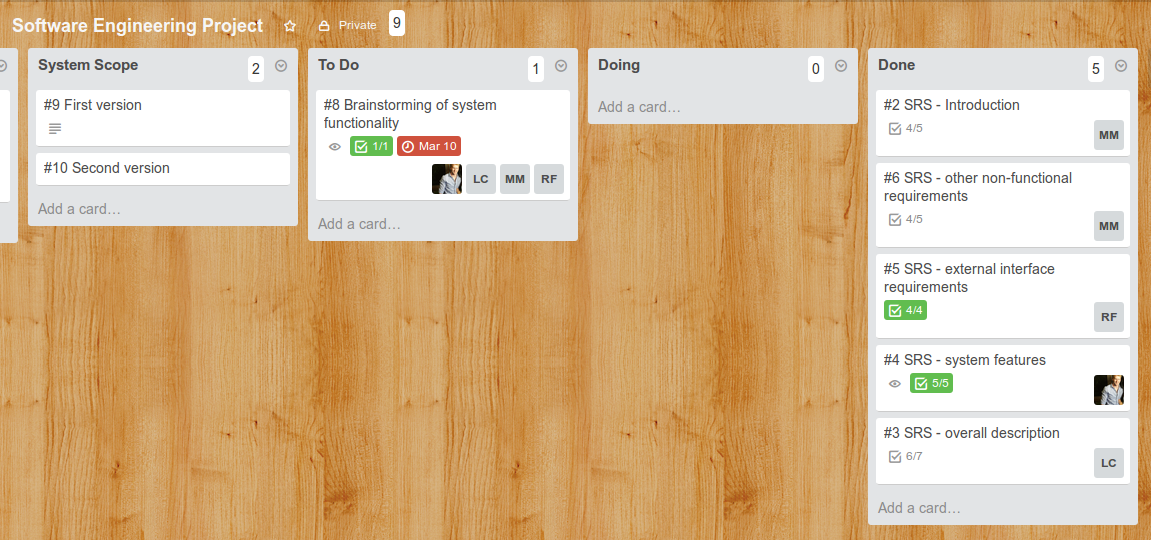
\includegraphics[scale = 0.45]{trello.png}
			\caption{Trello board used for project development}
			\label{menu}
		\end{figure}
	
	
\end{document}